\chapter{和积算法与滑动窗口解码的简介}
\section{LDPC分组码的和积算法}
和积算法是一种软判决算法。在算法迭代过程中,校验节点生成独立于信息节点接收到信息的额外信息,进而决定信息节点的值。以下介绍基本的和积算法。

记信源发送码字为$\mathbf{c}$,接收到的向量为$\mathbf{y}$。
将从校验节点$j$到它所连接信息节点$i$额外信息记为$E_{j,i}$。
如果某次迭代中,码字中$c_{i'}=1$的概率为$P_{j,i'}$,那么校验方程中包含奇数个$1$的概率为
\[
P_{j,i}^{ext} = \frac{1}{2} - \frac{1}{2} \prod_{i' \in B_j, i' \neq i} (1-2P_{j,i'})
\]
其中,$B_j$为与校验节点$j$相连的信息节点的下标集合。类似的,校验方程满足$c_{i}=0$时概率为$1-P_{j,i}^{ext}$。

校验节点$j$到信息节点$i$的额外信息用似然比来表示
\begin{eqnarray}
E_{j,i} & = & L(P_{j,i}^{ext})\\
& = & \text{log} \frac{1-P_{j,i}^{ext}}{P_{j,i}^{ext}}\\
& = & 2 \text{tanh}^{-1} \prod_{i' \in B_j, i' \neq i} \text{tanh} (M_{j,i'}/2)
\end{eqnarray}
其中
\[
M_{j,i'} \stackrel{\triangle}{=} L(P_{j,i'}) = \text{log} \frac{1-P_{j,i'}}{P_{j,i'}}
\]
每个信息节点接收输入的LLR,记为$R_i$
\[
R_i= \text{log} \frac{p(\mathbf{c}_i=0|y_i)}{p(\mathbf{c}_i=1|y_i)}
\]
同时接收来自相连接的校验节点的LLR。故信息节点$i$总的LLR为
\[
L_i = L(P_i) = R_i + \sum_{j\in A_i}E_{j,i}
\]
对于从信息节点发送到校验节点的信息,记为$M_{j,i}$
\[
M_{j,i}= R_i + \sum_{j' \in A_i,j'\neq j}E_{j',i}
\]
和积算法的具体步骤为
\begin{enumerate}
\item 给信息节点发送到校验节点的信息$M_{j,i}$赋值为$R_i$
\item 计算校验节点发送到信息节点的信息$E_{j,i}$
\item 计算信息节点的LLR,$L_i$。生成预测码字$\hat{c}$,代入校验方程,若满足,则停止算法。或者达到最大遍历值停止算法。
\item 计算信息节点发送到校验节点的信息$M_{j,i}$,遍历次数加一。继续第二步。
\end{enumerate}
如果该算法收敛,经过足够多次迭代后,将渐近求出码字中各位为1或者0的概率。实现逐符号最大后验概率译码。
\section{LDPC卷积码的滑动窗口解码}

\begin{center}
\def\linkdoub{\draw [double distance=1mm, very thick] (0,0)--}
\def\linksing{\draw [very thick] (0,0)--}
\def\check{%
    \filldraw [fill=white,very thick] (0,0) circle (5pt);
    \draw [very thick] (0,3.5pt)--(0,-3.5pt);
    \draw [very thick] (3.5pt,0)--(-3.5pt,0);
}
\def\bit{%
    \filldraw [fill=white,very thick] (0,0) circle (5pt);
    \draw [very thick] (-3.2pt,2.2pt)--(3.2pt,2.2pt);
    \draw [very thick] (-3.2pt,-2.2pt)--(3.2pt,-2.2pt);
}
\def\thetaone{60}
\def\thetatwo{-60}
\def\armLength{0.9}
\def\symbolDist{1}

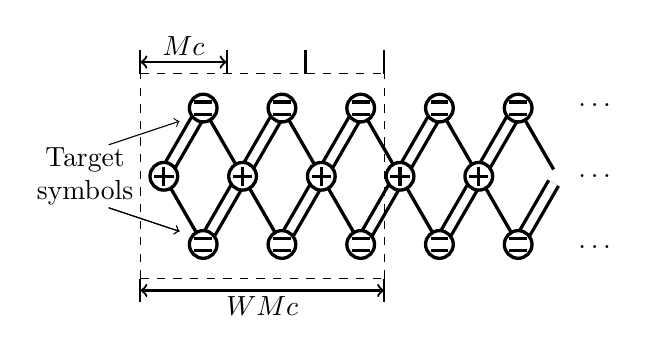
\begin{tikzpicture}
\foreach \x in {1,2,...,5}
{
	\begin{scope}[shift=(0:\x)]
		\linkdoub(\thetaone:\armLength);
		\linksing(\thetatwo:\armLength);
		\check
		\begin{scope}[shift=(\thetaone:\symbolDist)]
		\linksing(\thetatwo:\armLength);
		\bit
		\end{scope}
		\begin{scope}[shift=(\thetatwo:\symbolDist)]
		\linkdoub(\thetaone:\armLength);
		\bit
		\end{scope}
	\end{scope}
}
\node at (6.5,0.9) {\ldots};
\node at (6.5,0) {\ldots};
\node at (6.5,-0.9) {\ldots};
\node [align=center] at (0,0) {Target\\
symbols
};
\draw [->] (0.3,0.4) -- (1.2,0.7);
\draw [->] (0.3,-0.4) -- (1.2,-0.7);
\draw [->] (0.3,-0.4) -- (1.2,-0.7);
\draw [dashed] (0.7,-1.3) -- (3.8,-1.3);
\draw [dashed] (0.7,1.3) -- (3.8,1.3);
\draw [dashed] (0.7,-1.3) -- (0.7,1.3);
\draw [dashed] (3.8,-1.3) -- (3.8,1.3);
\draw [thick] (0.7,1.3) -- (0.7,1.6);
\draw [thick] (1.8,1.3) -- (1.8,1.6);
\draw [thick] (2.8,1.3) -- (2.8,1.6);
\draw [thick] (3.8,1.3) -- (3.8,1.6);
\draw [<->,thick] (0.7,1.45) -- (1.8,1.45);
\node [align=center] at (1.25,1.65) {$Mc$};
\draw [thick] (0.7,-1.3) -- (0.7,-1.6);
\draw [thick] (3.8,-1.3) -- (3.8,-1.6);
\draw [<->,thick] (0.7,-1.45) -- (3.8,-1.45);
\node [align=center] at (2.25,-1.65) {$WMc$};
\end{tikzpicture}
\figurecaption{滑动窗口解码器的例子,$t=0$}

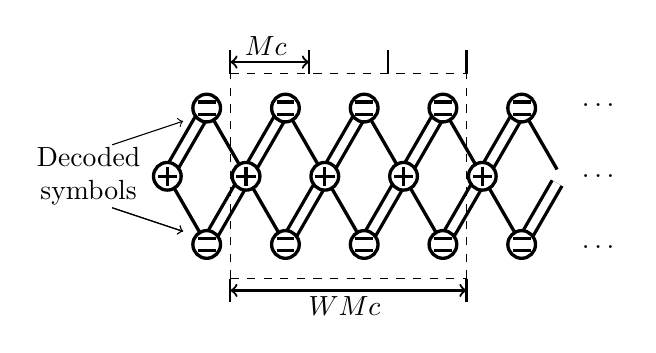
\begin{tikzpicture}
\foreach \x in {1,2,...,5}
{
	\begin{scope}[shift=(0:\x)]
		\linkdoub(\thetaone:\armLength);
		\linksing(\thetatwo:\armLength);
		\check
		\begin{scope}[shift=(\thetaone:\symbolDist)]
		\linksing(\thetatwo:\armLength);
		\bit
		\end{scope}
		\begin{scope}[shift=(\thetatwo:\symbolDist)]
		\linkdoub(\thetaone:\armLength);
		\bit
		\end{scope}
	\end{scope}
}
\node at (6.5,0.9) {\ldots};
\node at (6.5,0) {\ldots};
\node at (6.5,-0.9) {\ldots};
\node [align=center] at (0,0) {Decoded\\
symbols
};
\draw [->] (0.3,0.4) -- (1.2,0.7);
\draw [->] (0.3,-0.4) -- (1.2,-0.7);
\draw [->] (0.3,-0.4) -- (1.2,-0.7);
\draw [dashed] (1.8,-1.3) -- (4.8,-1.3);
\draw [dashed] (1.8,1.3) -- (4.8,1.3);
\draw [dashed] (1.8,-1.3) -- (1.8,1.3);
\draw [dashed] (4.8,-1.3) -- (4.8,1.3);
\draw [thick] (1.8,1.3) -- (1.8,1.6);
\draw [thick] (2.8,1.3) -- (2.8,1.6);
\draw [thick] (3.8,1.3) -- (3.8,1.6);
\draw [thick] (4.8,1.3) -- (4.8,1.6);
\draw [<->,thick] (1.8,1.45) -- (2.8,1.45);
\node [align=center] at (2.25,1.65) {$Mc$};
\draw [thick] (1.8,-1.3) -- (1.8,-1.6);
\draw [thick] (4.8,-1.3) -- (4.8,-1.6);
\draw [<->,thick] (1.8,-1.45) -- (4.8,-1.45);
\node [align=center] at (3.25,-1.65) {$WMc$};
\end{tikzpicture}
\figurecaption{滑动窗口解码器的例子,$t=1$}
\end{center}
上图为滑动窗口解码器的一个例子。其窗口大小为$W=3$,作用在$m_s=1$的(3,6)-正则$q$元LDPC卷积码上。
对于窗口里的$WMc$个符号,解码算法不断迭代,直到某一固定迭代次数或者满足某些停止规则。然后窗口平移$Mc$个位置,即已解码的$Mc$个符号从窗口移出。滑动窗口解码的解码延时为
\[
T_{CC} = WMmc
\]
因此,对于本文构造的LDPC分组码与LDPC卷积码,LDPC卷积码的解码延时$T_{CC}$等于LDPC分组码的码长,即等于LDPC分组码的解码延时$T_{BC}$。
滑动窗口解码器的窗口内迭代算法可以使用以上的和积算法,也可以用和积算法的改进版本\parencite{Barnault2003Fast}等。
窗口内迭代算法的停止规则如下。给定LDPC卷积码以及接收到的码字,令$P_t^{(j)}(b)$为在时刻$t$,窗口中第$j$个符号$v_t^{(j)}$的$b\in \text{GF} (q)$的概率。经过每次和积算法的迭代,基于$P_t^{(j)}(b)$对$v_t^{(j)}$进行硬判决,记为$\hat{v}_t^{(j)}$,即选择$\hat{v}_t^{(j)}=x$使得概率为最大值。记$e_t^{(j)}$为$v_t^{(j)}$不等于$\hat{v}_t^{(j)}$的概率,则
\[
e_t^{(j)}=1-P_t^{(j)}(x=\hat{v}_t^{(j)})
\]
而对于整个窗口内的符号,$e_t^{(j)}$的平均值为
\[
\hat{P}_t = \frac{1}{Mc}\sum_{j=0}^{Mc-1}e_t^{(j)}
\]
当迭代次数达到最大值$I_{max}$,或者$\hat{P}_t$小于某个选定的误符号率时,解码窗口才平移到下一个位置。